\section{Dinámica de los instrumentos indicadores}
\label{sec:dinamica}

Un instrumento analógico se compone de dos partes: una fija (estator) y una móvil (rotor). 
El principio es físico es simple: una fuerza (dependiente de la magnitud eléctrica a medir) empuja al rotor, produciendo un giro. A la relación entre lo que medimos y cuánto gira la aguja se le llama \emph{ley del instrumento}.

Resumen de los principales tipos de instrumentos y sus leyes de respuesta:

\begin{description}
  \item \textbf{Imán permanente y bobina móvil (PMMC)}
    \begin{itemize}
      \item \textit{Mide:} Corriente y tensión en \textbf{C.C.}
      \item \textit{Ley:} Lineal (\(\theta = K \cdot i\)).
    \end{itemize}
  \item \textbf{Hierro móvil}
    \begin{itemize}
      \item \textit{Mide:} Corriente y tensión en \textbf{C.C. y C.A.}
      \item \textit{Ley:} Cuadrática (\(\theta = \frac{dL}{d\theta}I^2\)).
    \end{itemize}
  \item \textbf{Electrodinámico}
    \begin{itemize}
      \item \textit{Mide:} Pohencia, corriente, tensión.
      \item \textit{Ley:} Depende del coseno de fase (\(\theta = \frac{dM}{d\theta}I_fI_m \cos(\beta)\)).
    \end{itemize}
  \item \textbf{Inducción}
    \begin{itemize}
      \item \textit{Mide:} Energía (medidores de luz) y potencia en \textbf{C.A.}
      \item \textit{Ley:} Depende del seno (\(\theta = K I_1 I_2 \sin(\beta)\)).
    \end{itemize}
\end{description}

\subsection{Ecuación general del movimiento (Las Cuplas)}

Para entender la dinámica, definiremos las fuerzas de rotación (Torques) como \textbf{Cuplas}. Para que la aguja se detenga en el valor correcto, deben interactuar tres tipos de cuplas:

\begin{enumerate}
    \item \textbf{Cupla Motora (\(C_m\)):} Es la fuerza que quiere mover la aguja. Su origen es eléctrico (magnético, electrostático, etc.).
    \item \textbf{Cupla Antagónica o Directriz (\(C_d\)):} Es la fuerza que ``tira hacia atrás''. Generalmente es un resorte que se retuerce. Si no existiera, la aguja daría vueltas completas como un motor.
    \item \textbf{Cupla de Amortiguamiento (\(C_a\)):} Es el freno. Solo aparece cuando hay movimiento y evita que la aguja oscile eternamente alrededor del valor final.
\end{enumerate}

La ecuación diferencial que describe el equilibrio dinámico es:
\[ C_m = C_d + C_a + C_i \]
Donde \(C_i\) es la inercia del sistema (\(J \frac{d^2\theta}{dt^2}\)).

\subsection[Análisis de la Cupla Directriz]{Análisis de la Cupla Directriz (\(C_d\))}

La cupla directriz (o de restitución) suele generarse mediante resortes en espiral o cintas de torsión. Su fuerza es proporcional al ángulo girado (Ley de Hooke angular):
\[ C_d = K_r \cdot \theta \]
Donde \(K_r\) depende del material (bronce-fosforoso) y la geometría del resorte.

\subsubsection{El proceso de equilibrio}
Imaginemos que conectamos el instrumento. La aguja empieza en cero:
\begin{enumerate}
    \item Al principio, la \textbf{Cupla Motora} es máxima y la \textbf{Antagónica} es cero. La aguja acelera.
    \item A medida que la aguja gira (\(\theta\) crece), el resorte se tensa y la Cupla Antagónica aumenta, oponiéndose al movimiento.
    \item El equilibrio se alcanza teóricamente cuando ambas fuerzas se igualan: \(C_m = C_d\).
\end{enumerate}

El gráfico de la figura \ref{fig_cuplas_instrumentales} ilustra cómo la Cupla Directriz (\(C_d\), línea roja) crece linealmente hasta cruzar las líneas de Cupla Motora (\(C_{m1}, C_{m2}\)), determinando los ángulos de equilibrio \(\theta_1\) y \(\theta_2\).

\begin{figure}[ht]
  \centering
  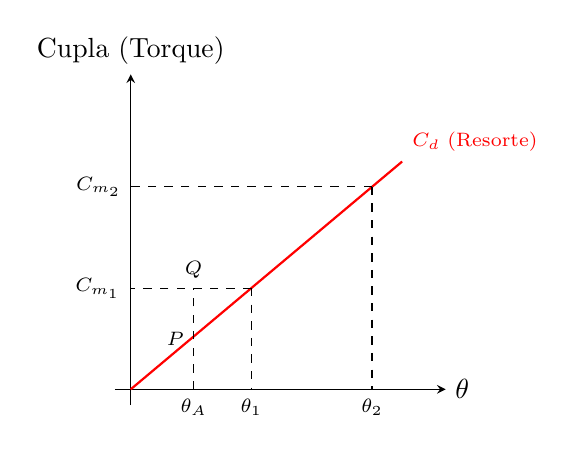
\begin{tikzpicture}[>=stealth]
    % Axis
    \draw[->] (-0.2,0) -- (4,0) node[right] {\(\theta\)};
    \draw[->] (0,-0.2) -- (0,4) node[above] {Cupla (Torque)};

    % cd curve (Linear Spring)
    \draw[red,thick] (0,0) -- (40:4.5) node[above right] {\scriptsize{\(C_d\) (Resorte)}};

    % intersections to cd (Equilibrium points)
    \draw[dashed] (40:2) -- ++(-1.54,0) node[left] {\scriptsize{\(C_{m_1}\)}};
    \draw[dashed] (40:4) -- ++(-3.06,0) node[left] {\scriptsize{\(C_{m_2}\)}};
    
    % Dropping lines to alpha axis
    \draw[dashed] (40:2) -- ++(0,-1.29) node[below] {\scriptsize{\(\theta_1\)}};
    \draw[dashed] (40:4) -- ++(0,-2.57) node[below] {\scriptsize{\(\theta_2\)}};
    
    % Visualizing the forces
    \draw[dashed] (0.8,0) node[below]{\scriptsize{\(\theta_A\)}} -- node[left]{\scriptsize{\(P\)}} (0.8,1.29) node[above]{\scriptsize{\(Q\)}};
  \end{tikzpicture}
  \caption{Interacción entre Cupla Motora (horizontal) y Directriz (diagonal). El punto de cruce es la lectura final.}
  \label{fig_cuplas_instrumentales}
\end{figure}

\subsection[Cuplas de amortiguamiento]{Cuplas de Amortiguamiento (\(C_a\))}

Esta cupla es necesaria para disipar la energía cinética. Sin ella, la aguja oscilaría mucho tiempo antes de detenerse. Existen tres tipos principales:

\subsubsection{1. Amortiguamiento por Rozamiento Sólido (Indeseable)}
Es el roce entre el eje y los pivotes. \textbf{Es malo} porque introduce un error: la aguja se detiene un poco antes o un poco después del valor real (zona de incertidumbre \(\delta\)).

\subsubsection{2. Amortiguamiento Fluido (Por aire)}
Se usa un aspa moviéndose dentro de una cámara cerrada (como un pistón de aire). Es común en instrumentos de Hierro Móvil.

\subsubsection{3. Amortiguamiento Magnético (Frenado por Corrientes de Foucault)}
Es el más efectivo y elegante. Se basa en la Ley de Lenz: \emph{``El movimiento induce una corriente que se opone a la causa que lo produce''}.

\textbf{¿Cómo funciona paso a paso?} 
\begin{enumerate}
    \item Un disco (o bobina) de aluminio conductor se mueve a velocidad \(v\) dentro de un campo magnético \(B\).
    \item Se induce una fuerza electromotriz (f.e.m.): \( e = B \cdot l \cdot v \).
    \item Como el material es conductor, circula una corriente: \( i = e / R \).
    \item Esta corriente interactúa con el imán creando una fuerza de frenado: \( F = B \cdot l \cdot i \).
\end{enumerate}

Sustituyendo las ecuaciones, obtenemos que el torque de frenado es proporcional a la velocidad angular \(\omega\):
\[ C_a = \left( \frac{B^2 l^2 r^2}{R} \right) \cdot \omega = D \cdot \omega \]
Donde \(D\) es la constante de amortiguamiento. Para que frene bien, necesitamos baja resistencia \(R\) (por eso usamos aluminio) y un campo magnético \(B\) fuerte.

\textbf{Caso especial: Bobina Móvil}
En los instrumentos de bobina móvil, la propia bobina actúa como freno si el circuito externo es de baja resistencia. Además, la bobina suele enrollarse sobre un marco de aluminio. El frenado total es la suma de dos efectos:
\[ D_{\text{total}} = D_{\text{bobina}} + D_{\text{marco aluminio}} \]
\[ D = B^2 l^2 a^2 \left( \underbrace{\frac{N^2}{R}}_{\text{Circuito}} + \underbrace{\frac{S_{Al}}{2\rho(l+a)}}_{\text{Marco de Al}} \right) \]

Todos estos sistemas de amortiguamiento, y cuplas se encuentran materializados en el instrumento como se muestra en la figura \ref{fig_galvanometro}, que ilustra un galvanómetro de imán permanente y bobina móvil.

\begin{figure}[ht]
  \centering
  \includegraphics[height=7cm]{chapters/1_unit/media/bin/galvanometro.pdf}
  \caption{Galvanómetro de imán permanente y bobina móvil.}
  \label{fig_galvanometro}
\end{figure}

\subsection{Sistemas de Suspensión}
Para minimizar el error por rozamiento sólido, se utilizan pivotes de alta calidad (piedras preciosas) o, en instrumentos de alta precisión, suspensión por \textbf{cinta tensa}, que elimina totalmente la fricción mecánica al hacer flotar el sistema móvil .

\section{Estudio de la ecuación del movimiento}

El comportamiento dinámico de un instrumento indicador analógico se modela considerando el sistema móvil como un cuerpo rígido con un solo grado de libertad: la rotación alrededor de su eje. Aplicando la segunda ley de Newton para la rotación, la suma de las cuplas actuantes debe igualar al momento de inercia (\(J\)) por la aceleración angular (\(\ddot{\theta}\))\footnote{Se ha usado la notación de Newton para las derivadas: \(\ddot{\theta}=\theta''\)}:

\[
  \sum C = C_m - C_d - C_a = J \frac{d^2\theta}{dt^2}
\]

Reemplazando cada cupla por su expresión constitutiva (donde \(D\) es la constante de amortiguamiento y \(K\) la del resorte), y reordenando, obtenemos la ecuación diferencial de segundo orden que rige el movimiento:

\begin{equation}\label{eq:edo_instrumento}
  J\frac{d^2\theta}{dt^2} + D\frac{d\theta}{dt} + K\theta = C_m
\end{equation}

Esta ecuación nos dice que la energía entregada por la cupla motora \(C_m\) se distribuye en vencer la inercia, la fricción (amortiguamiento) y la restitución del resorte.

\subsection{Respuesta transitoria y regímenes de movimiento}

La solución de la ecuación \eqref{eq:edo_instrumento} se compone de dos partes: \(\theta(t) = \theta_p + \theta_h(t)\).
\begin{itemize}
    \item \textbf{Solución Permanente (\(\theta_p\)):} Es la posición final de equilibrio donde la aguja se detiene. Se obtiene cuando las derivadas temporales son nulas: \(\theta_p = C_m / K\).
    \item \textbf{Solución Transitoria (\(\theta_h\)):} Describe la trayectoria de la aguja desde el cero hasta \(\theta_p\). Su comportamiento depende de las raíces de la ecuación característica (\(Jr^2 + Dr + K = 0\)).
\end{itemize}

Dependiendo de la magnitud del amortiguamiento \(D\) respecto a la inercia y el resorte, definimos el \emph{factor de amortiguamiento}. Esto da lugar a tres casos físicos claramente diferenciados:

\begin{enumerate}
  \item \textbf{Movimiento Subamortiguado (Oscilatorio)} \\
  Ocurre cuando el amortiguamiento es pequeño (\(\frac{D^2}{4J^2} < \frac{K}{J}\)). Las raíces son complejas conjugadas.
  
  La aguja sobrepasa el valor final \(\theta_p\) y oscila alrededor de él con una amplitud que decrece exponencialmente hasta detenerse.
  
  \begin{figure}[!ht]
    \centering
    \includegraphics[width=7cm]{chapters/1_unit/media/bin/amortiguamiento.png}
    \caption{Respuesta subamortiguada: la aguja oscila antes de detenerse.}
    \label{fig:subamortiguamiento}
  \end{figure}

  \emph{Importancia práctica:} La mayoría de los instrumentos se diseñan para ser \textbf{ligeramente subamortiguados}. Esa pequeña oscilación inicial asegura al operador que el sistema móvil no está atascado por rozamiento estático (fricción en los pivotes).

  \item \textbf{Movimiento Crítico} \\
  Ocurre en el límite matemático exacto donde las raíces son reales e iguales (\(\frac{D^2}{4J^2} = \frac{K}{J}\)).
  
  Es la condición teórica donde la aguja llega al valor final en el \textbf{menor tiempo posible} sin sobrepasarlo (sin oscilar).

  \begin{figure}[!ht]
    \centering
    \includegraphics[width=7cm]{chapters/1_unit/media/bin/critico.png}
    \caption{Amortiguamiento crítico: respuesta más rápida sin sobrepaso.}
    \label{fig:critico}
  \end{figure}
  
  Aunque parece ideal por su velocidad, es difícil de fabricar y mantener, ya que cualquier envejecimiento de los materiales podría llevar al instrumento al estado sobreamortiguado, volviéndolo lento.

  \item \textbf{Movimiento Sobreamortiguado (Aperiódico)} \\
  Ocurre cuando el amortiguamiento es excesivo (\(\frac{D^2}{4J^2} > \frac{K}{J}\)). Las raíces son reales y distintas.
  
  La aguja se aproxima al valor final \(\theta_p\) de manera asintótica y muy lenta. El sistema parece ``pesado'' o ``perezoso''.
  
  \begin{figure}[!ht]
    \centering
    \includegraphics[width=5cm]{chapters/1_unit/media/bin/sobreamortiguado.png}
    \caption{Respuesta sobreamortiguada: aproximación lenta.}
    \label{fig:sobreamortiguado}
  \end{figure}
  
  Este comportamiento es generalmente indeseable en instrumentos de medida, ya que obliga al operador a esperar demasiado tiempo para tomar una lectura confiable.
\end{enumerate}

\subsection{Respuesta a una excitación sinusoidal}

¿Qué sucede si la cupla motora no es constante, sino que varía sinusoidalmente en el tiempo (\(C_m = C_0 \sin(\omega t)\))? Esto ocurre al medir corriente alterna o señales variables. La ecuación diferencial se convierte en:

\[
  J\ddot{\theta} + D\dot{\theta} + K\theta = C_0 \sin(\omega t)
\]

La aguja intentará seguir el ritmo de la fuerza externa. Pasado el transitorio inicial, la aguja oscilará a la misma frecuencia \(\omega\) que la señal, pero con dos diferencias fundamentales:
\begin{enumerate}
    \item Cambio de Amplitud (\(A\)): La aguja puede moverse más o menos de lo que debería estáticamente.
    \item Desfase (\(\varphi\)): La aguja se moverá con un retraso respecto a la señal eléctrica.
\end{enumerate}

La solución estacionaria es:
\[
  \theta(t) = \theta_{\text{estática}} \cdot A \cdot \sin(\omega t - \varphi)
\]
Donde \(A\) es el \textbf{Factor de Amplificación Dinámica}. Su comportamiento depende de la relación entre la frecuencia de la señal (\(\omega\)) y la frecuencia natural del instrumento (\(\omega_0 = \sqrt{K/J}\)):

\begin{itemize}
    \item \textbf{Baja frecuencia (\(\omega \ll \omega_0\)):} El factor \(A \approx 1\). El instrumento sigue fielmente a la señal.
    \item \textbf{Resonancia (\(\omega \approx \omega_0\)):} El factor \(A\) se dispara (\(A \gg 1\)). La aguja oscila exageradamente aunque la señal sea pequeña.
    \item \textbf{Alta frecuencia (\(\omega \gg \omega_0\)):} El factor \(A \to 0\). La aguja no tiene tiempo de reaccionar debido a su inercia y se queda quieta.
\end{itemize}

\subsection{Aplicaciones y consecuencias prácticas}

Dependiendo de qué queramos medir, diseñaremos el instrumento para trabajar en una zona u otra de la curva de respuesta.

\subsubsection{1. Instrumentos Registradores (Fidelidad)}
Si queremos registrar una señal compleja (como un electrocardiograma o una onda sísmica), necesitamos que el dibujo sea una copia fiel de la realidad.
\begin{itemize}
    \item \textbf{Requisito:} Necesitamos que \(A \approx 1\) y que el retardo sea constante.
    \item \textbf{Solución:} El instrumento debe tener una frecuencia natural \(\omega_0\) muy alta (ser muy rápido y ligero) para que todas las frecuencias de la señal sean consideradas ``bajas'' (\(\omega \ll \omega_0\)).
\end{itemize}

\subsubsection{2. Galvanómetro de Vibración (Selectividad)}
\emph{Aclaración conceptual:} Imagina un columpio. Si lo empujas justo a su ritmo natural, oscila muy alto con poca fuerza.
Este instrumento aprovecha la resonancia. Se ajusta mecánicamente (tensando la suspensión) para que su frecuencia natural coincida exactamente con la frecuencia que queremos medir (ej. \qty{50}{\hertz}).
\begin{itemize}
    \item \textbf{Efecto:} Amplifica enormemente esa frecuencia específica (\(A \gg 1\)) y atenúa el resto. Funciona como un filtro mecánico de banda muy estrecha de alta sensibilidad.
\end{itemize}

\subsubsection{3. Distorsión en señales complejas}
Una señal no senoidal (como una onda cuadrada o triangular) es la suma de muchas ondas senoidales de distintas frecuencias (armónicos).
Si medimos esto con un instrumento lento:
\begin{enumerate}
    \item Los armónicos bajos se medirán bien (\(A \approx 1\)).
    \item Los armónicos altos se atenuarán (\(A < 1\)) y sufrirán mayor retraso (\(\varphi\)).
\end{enumerate}
El resultado es que la aguja dibujará una onda ``suavizada'' o deformada respecto a la original, perdiendo los detalles rápidos, como se ve en la figura \ref{fig:in_vs_out}.

\begin{figure}[!ht]
  \centering
  \includegraphics[height=5cm]{chapters/1_unit/media/bin/in_vs_out.png}
  \caption{Efecto de la inercia del instrumento: la señal de salida (azul/suave) pierde los detalles rápidos y llega retrasada respecto a la entrada (roja/brusca).}
  \label{fig:in_vs_out}
\end{figure}

\subsection{El filtrado mecánico en instrumentos de Ley Cuadrática}

\emph{Explicación del fenómeno:} En un instrumento electrodinámico (que mide potencia o corriente eficaz), la fuerza es proporcional al cuadrado de la corriente (\(F \propto i^2\)). Si la corriente es alterna (\(i = \sin(\omega t)\)), la fuerza es:
\[ i^2 = \sin^2(\omega t) = \frac{1}{2} - \frac{1}{2}\cos(2\omega t) \]
Esto significa que la fuerza tiene dos partes:
\begin{enumerate}
    \item Una componente constante (\(1/2\)): Que empuja la aguja hacia el valor a medir.
    \item Una componente vibratoria (\(2\omega\)): Que intenta hacer vibrar la aguja al doble de la frecuencia de la red (ej. \qty{100}{\hertz}).
\end{enumerate}

¿Por qué la aguja no vibra furiosamente? Porque para la aguja (que es un sistema mecánico con masa), \qty{100}{\hertz} es una frecuencia altísima (\(\omega \gg \omega_0\)).
Estamos en la zona donde \(A \to 0\). La inercia del instrumento filtra mecánicamente la vibración, y la aguja solo responde al componente constante promedio. Es decir, el instrumento calcula ``automáticamente'' el valor medio cuadrático gracias a que es incapaz de seguir la vibración rápida.
